\section{Aprendizaje Automático}

\note{Una vez que tenemos una idea general de lo que se quiere hacer y que tenemos un conjunto de datos para trabajar, procederíamos a mostrar nuestra implementación del clasificador. Pero antes es necesario estar en contexto sobre las técnicas utilizadas en este trabajo, que son del área \textbf{Aprendizaje Automático}.}

\begin{frame}
    \frametitle{Aprendizaje Automático}

    \begin{itemize}
        \item Objetivo: hacer \emph{aprender} a una computadora.
        \item Aprendizaje \emph{supervisado}.
        \item En la \emph{clasificación} se intenta aprender la categoría de una entidad.
    \end{itemize}
\end{frame}

\note{Aprendizaje Automático es un área que tiene como objetivo hacer \textbf{aprender} a una computadora.

A su vez nosotros nos vamos a concentrar en lo que es el aprendizaje \textbf{supervisado}, es decir, aprender en base a ejemplos claramente etiquetados. En nuestro caso se aprenderá en base a tweets etiquetados como Humor o como No humor.

La tarea particular que queremos realizar se llama \textbf{clasificación}, y esto es que queremos asignarle una etiqueta (Humor o No humor) a una instancia, a un tweet.}

\subsection{Clasificadores}
\begin{frame}
    \frametitle{Clasificadores}
    
    \begin{itemize}
        \item Un clasificador decide en base a \emph{características} y a ciertas suposiciones.
    \end{itemize}
\end{frame}

\note{En cuanto a los clasificadores, ellos deciden en base a \textbf{características}, a valores, y además hacen suposiciones para generalizar cómo se comporta lo que se quiere buscar, en este caso el humor.

A continuación vamos a mostrar 4 técnicas que usamos en este trabajo, que hacen suposiciones distintas.}

\begin{frame}
    \frametitle{Support Vector Machine (SVM)}

    \begin{center}
        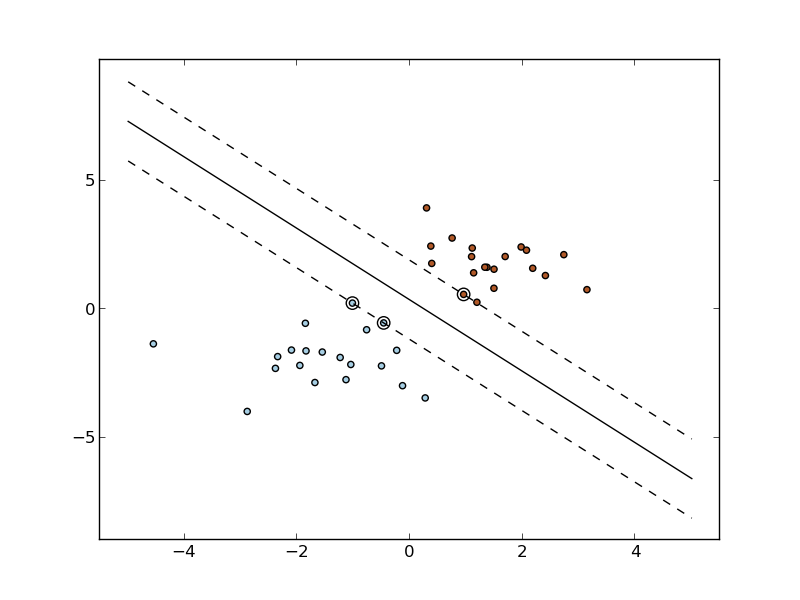
\includegraphics{svm.png}
    \end{center}
\end{frame}

\note{La primera técnica que mostramos es Suport Vector Machine o SVM. SVM se basa en primero pasar las instancias a un espacio vectorial, en donde cada componente de cada tweet tiene el valor de una característica. Por ejemplo un tweet puede tener 1 en Ambigüedad y 3,5 en Jerga sexual. SVM intenta buscar la curva que mejor separe los ejemplos de las distintas clases.

Se muestra un ejemplo acá. En este caso el espacio vectorial es un plano y la curva elegida es una recta. Los ejemplos en este caso quedaron completamente separados, y es lo que supone SVM, pero no siempre ocurre esto.}

\begin{frame}
    \frametitle{Árbol de decisión (DT)}

    \begin{center}
        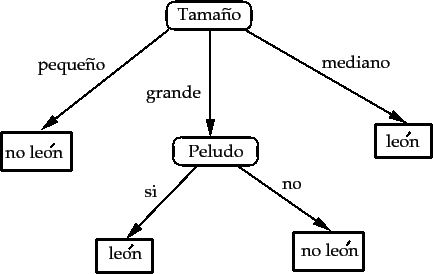
\includegraphics{dts.png}
    \end{center}
\end{frame}

\note{También usamos los Árboles de decisión. Ellos son estructuras en forma de árbol que en los nodos internos preguntan por atributos y en las ramas que salen de ellos se desprenden los valores posibles. En las hojas tienen categorías posibles.

El algoritmo de aprendizaje automático utilizado para armarlos se basa en la idea que las características más discriminantes deben ir más arriba en el árbol.

Mostramos un ejemplo, para contrastar con otras técnicas. En este clasificador para predecir una instancia se pregunta primero por si es ambiguo un tweet. Si lo es, se considera humorístico. Si no, se pregunta por el valor de Jerga sexual. Si es alto, es humorístico y sino es no humorístico.}

\begin{frame}
    \frametitle{Naïve Bayes (NB)}

    \begin{center}
        \begin{tabular}{c | c | c | c | c}
            & \multicolumn{2}{c |}{Ambigüedad} & \multicolumn{2}{c}{Jerga sexual} \\
            \hline
            & Sí & No & Alta & Baja \\
            \hline
            Humor & 0,90 & 0,10 & 0,80 & 0,20 \\
            \hline
            No humor & 0,30 & 0,70 & 0,25 & 0,75 \\
        \end{tabular}

        \vfill

        Un tweet es apriori igual de probable de ser humor o no.

        \vfill

        ¿Si tengo un tweet ambiguo y con jerga sexual?

        \vfill

        \small
        \begin{align*}
            P(Ambiguedad=Si|Humor) \times P(Jerga sexual=Alta|Humor) &= 0.72 \\
            P(Ambiguedad=Si|No\ humor) \times P(Jerga sexual=Alta|No\ humor) &= 0.075
        \end{align*}
    \end{center}
\end{frame}

\note{Por otro lado están los clasificadores bayesianos ingenuos. Se basan en el Teorema de Bayes.

Los mostramos con el siguiente ejemplo. Supongamos que tenemos que hay alta probabilidad de que un tweet humorístico sea ambiguo y tenga jerga sexual, y que si no es humorístico es baja en general. ¿Qué pasaría si tenemos un tweet ambiguo y con altos valores de Jerga sexual, suponiendo que estamos en un mundo con a priori igual cantidad de humor y tweets no humorísticos? Mirando las probabilidades por separado de cada características podemos obtener la categoría más probable.

Naïve Bayes hace esto: mira las probabilidades de cada característica según cada categoría para decidir.}

\begin{frame}
    \frametitle{k Nearest Neighbors (kNN)}

    \begin{center}
        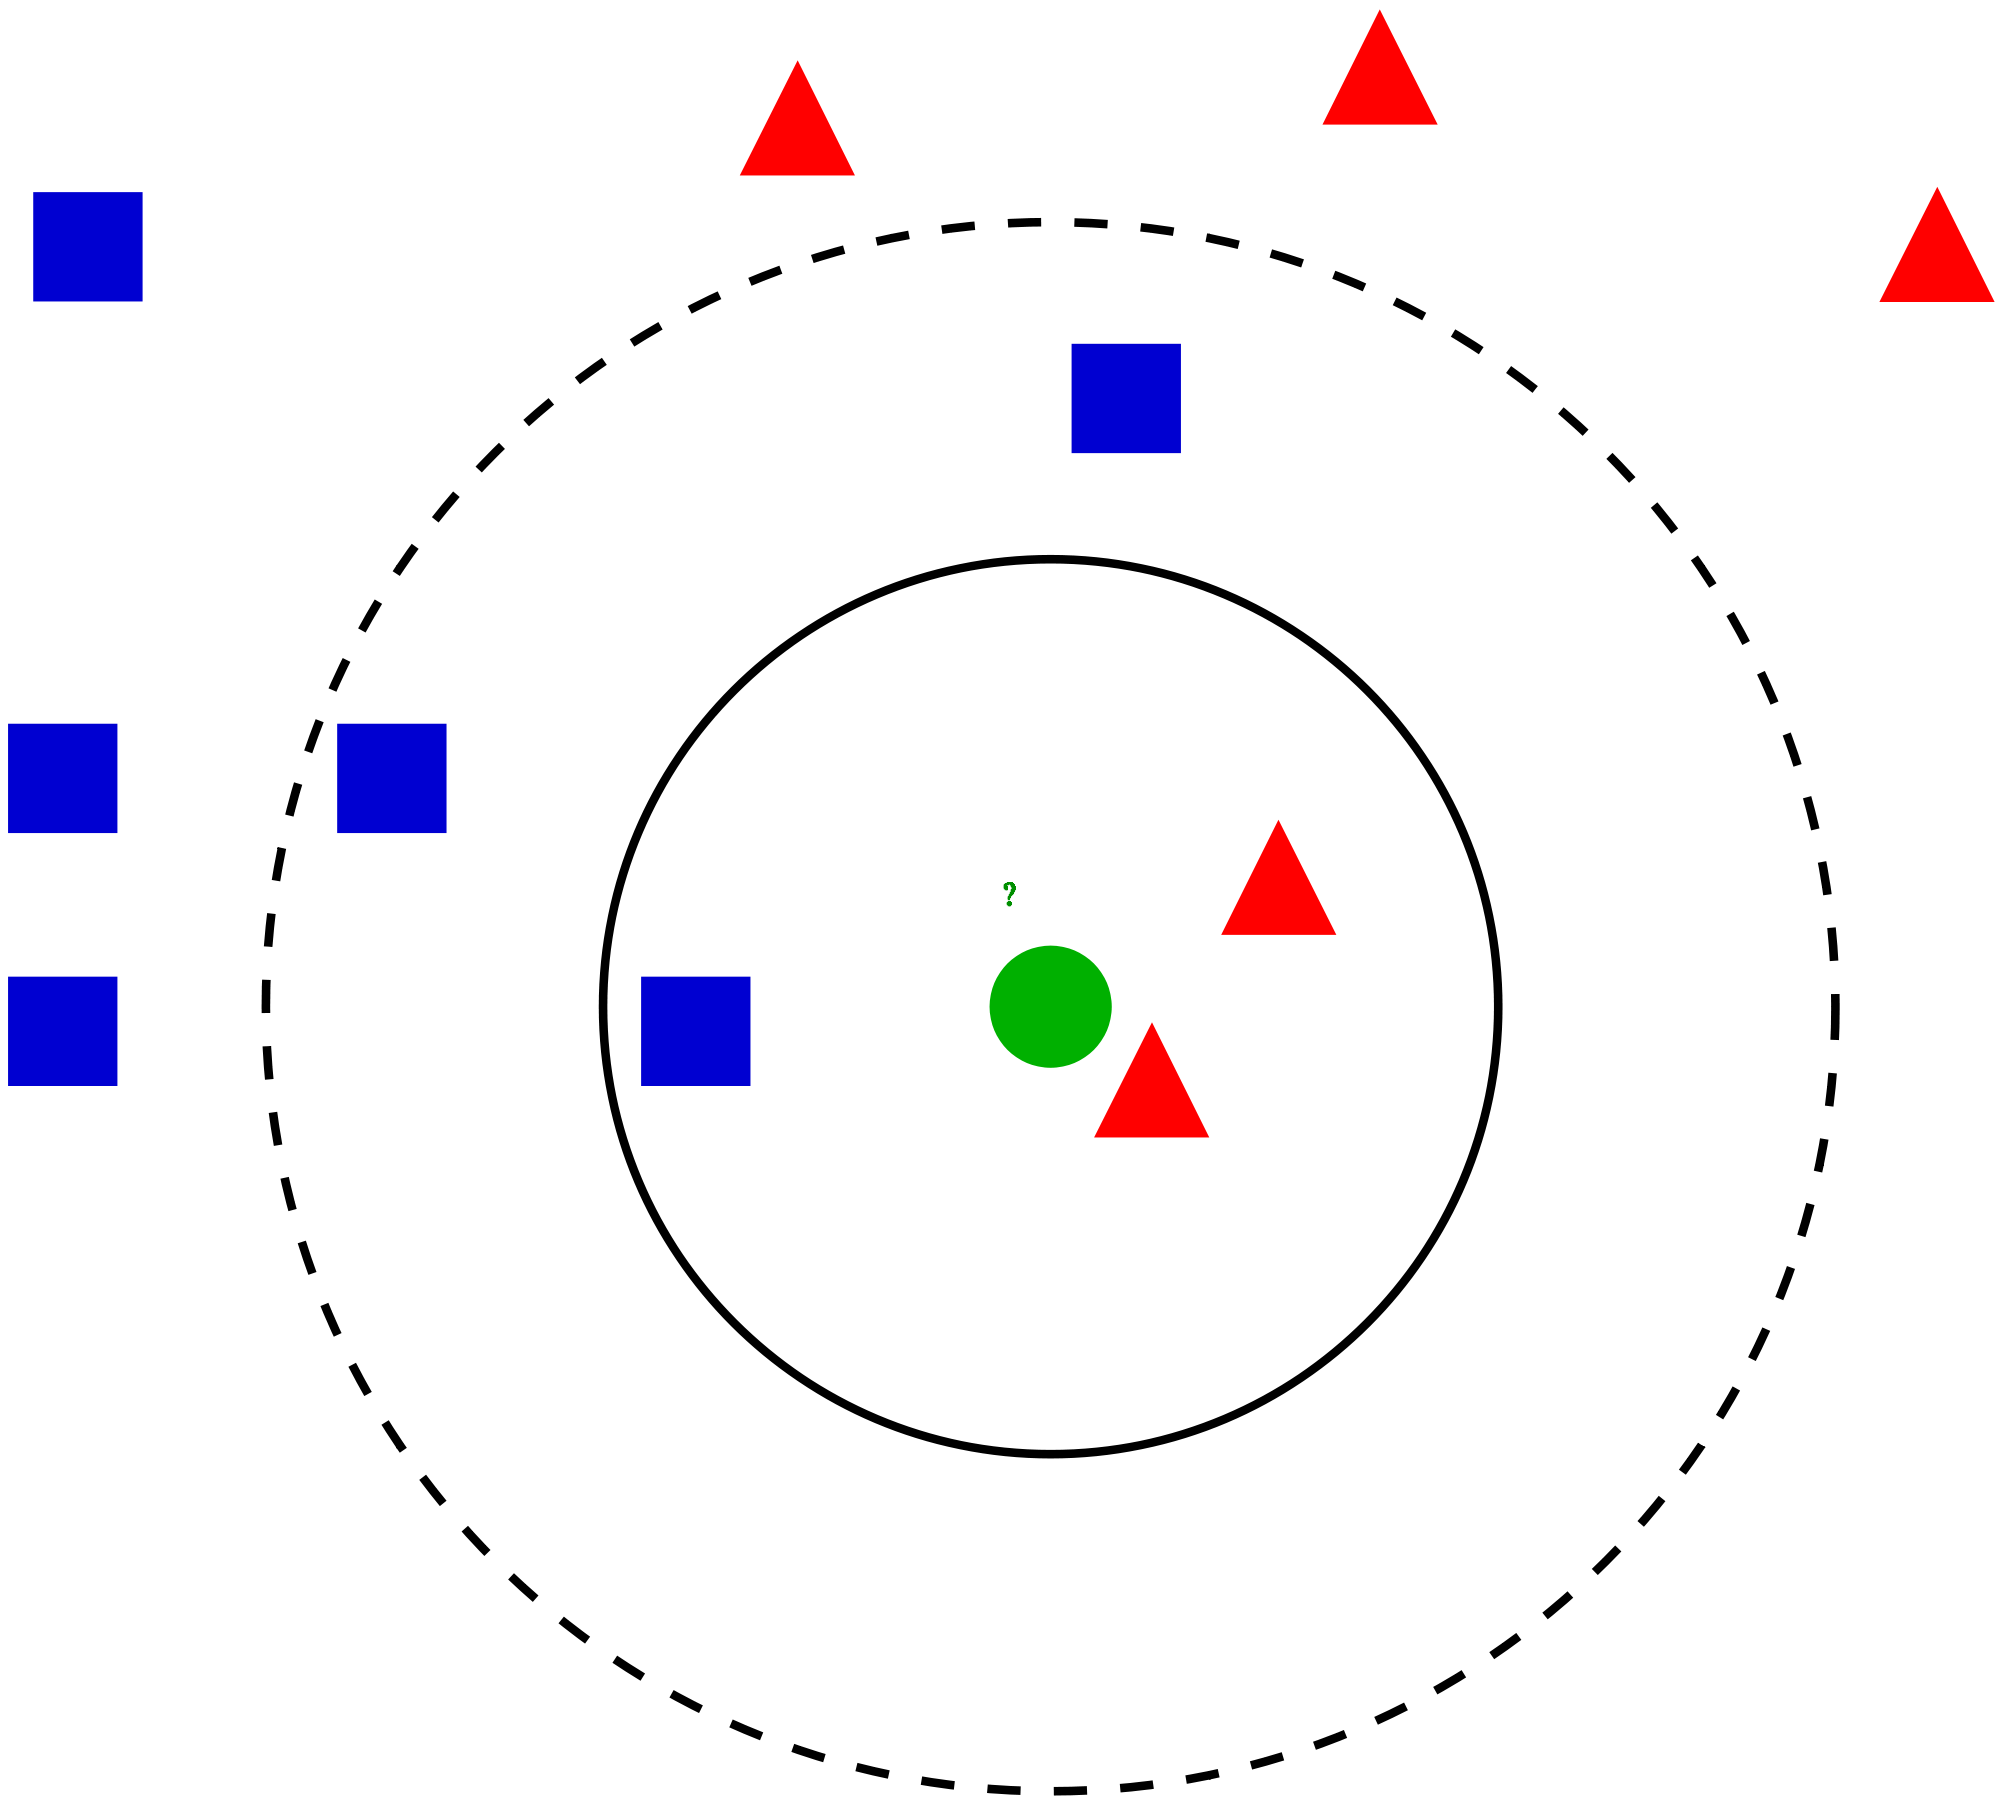
\includegraphics{knn.png}
    \end{center}
\end{frame}

\note{Por último está \textbf{k Nearest Neighbors} (kNN), o los \emph{k} vecinos más cercanos, que es un tipo de clasificador que para predecir el valor de una instancia mira otras consideradas cercanas. De manera similar a SVM usa un espacio vectorial para representar las instancias. El dibujo ilustra que se quiere clasificar el círculo como rojo o azul. Mirando las tres más cercanas, se da por rojo, aunque las cinco más cercanas da por ejemplo azul.

Siguiendo el ejemplo de los tweets, se podría predecir una instancia en base a tweets con valores de Ambigüedad y Jerga sexual parecidos.}

\subsection{Metodología}
\begin{frame}
    \frametitle{Metodología}

    \begin{itemize}
        \item Entrenamiento y evaluación
    \end{itemize}
\end{frame}

\note{
    ¿Qué metodología se lleva a cabo? Usualmente se separa en etapas de Entrenamiento y Evaluación. Primero se dividen los datos en conjunto de entrenamiento y conjunto de evaluación. Con la primera parte se ajusta el algoritmo, y los parámetros de la técnica utilizada. Luego se utiliza el conjunto de evaluación para tomar medidas del clasificador, para ver qué tan bien le va a la hora de predecir y para poder compararlo con otros.
}

\subsection{Métricas}
\begin{frame}
    \frametitle{Métricas}
    
    \begin{columns}[T]
        \begin{column}[T]{.4\textwidth}
            \begin{block}{Tipos de instancias}
                \begin{itemize}
                    \item Verdaderos positivos
                    \item Falsos positivos
                    \item Falsos negativos
                    \item Verdaderos negativos
                \end{itemize}
            \end{block}

            \begin{block}{Medidas}
                \begin{itemize}
                    \item Precisión, $P = \frac{VP}{VP + FP}$
                    \item Recall, $R = \frac{VP}{VP + FN}$
                    \item $F_1 = \frac{2 P R}{P + R} = \frac{VP}{VP + \frac{FP + FN}{2}}$
                    \item Acierto $= \frac{VP + VN}{VP + VN + FP + FN}$
                \end{itemize}
            \end{block}
        \end{column}

        \begin{column}[T]{.6\textwidth}
            \begin{center}
                \includesvg[height=7cm, svgpath=imagenes/]{medidas}
            \end{center}
        \end{column}
    \end{columns}
\end{frame}

\note{
    Es importante contar con medidas para poder evaluar el desempeño de un aprendiz y poder compararlo con otros, como dijimos.

    Supongamos primero que queremos distinguir los círculos (que son los positivos) de las circunferencias (que son los negativos). Recordemos que en nuestro caso positivo es igual a Humor. En el ejemplo la solución se encuentra al mirar las figuras a uno y otro lado de la línea recta. Pero el clasificador del ejemplo considera como positivos a los que se encuentran dentro de la elipse.

    Es necesario distinguir a las instancias según el tipo de resultado obtenido al predecir. Los verdaderos y falsos positivos [mostrar en la imagen] son aquellos considerados como positivos por el clasificador de manera correcta y de manera incorrecta respectivamente. De manera similar tenemos los verdaderos y falsos negativos [mostrar en la imagen], es decir los considerados negativos por el clasificador correcta e incorrectamente clasificados.
}

\note{
    A partir de lo anterior, se definen 4 medidas. \textbf{Precisión} (ilustrada por la P en el dibujo) es la fracción de instancias correctamente etiquetadas como positivas según todas las consideradas positivas. Es la relación entre la parte verde de la elipse y la elipse en sí. Presta atención a los errores de falso positivo. El \textbf{Recall} (ilustrado por la R en el dibujo) mide la relación entre los correctamente encontrados respecto a todos los que positivos había. De esta manera presta atención a los errores de tipo II (falsos negativos). La medida \textbf{$F_1$} es muy similar a las anteriores, pero pondera de igual manera los dos tipos de errores. Se puede ver como una medida promedio de las anteriores también.

    Notar que estas medidas le prestan atención a los positivos. Si se quiere hacer lo mismo con los negativos, basta con dar vuelta los roles positivo-negativo.

    A su vez está el \textbf{Acierto}, que es el porcentaje de instancias correctamente clasificadas, de cualquier tipo.
}
